\documentclass[a4paper, 11pt]{article}

\usepackage[T1]{fontenc}
\usepackage[utf8]{inputenc}

\usepackage{graphicx}

\usepackage{microtype}

\usepackage{xcolor}

\title{Aprendizaje Automático \\ Trabajo Práctico 1 --- Detección de Spam}
\author{Martín Fixman \and Leandro Matayoshi \and Fernando Gasperi}
\date{Segundo Cuatrimestre de 2016}

\newcommand{\todox}{\(\mathit{\color{red}x}\)}

\newcommand{\ham}{\large{\texttt{ham}}}
\newcommand{\spam}{\large{\texttt{spam}}}

\begin{document}
\maketitle

\newpage

\section{Extracción de Atributos}

\section{Selección de Modelos}

En el punto anterior logramos conseguir una \textbf{Matriz de Features} \( X \), con \todox{} columnas (features) y \todox{} filas (samples), y un vector de clases \( y \) con \todox{} samples, donde cada una índica si cada sample debería pertenecer a \ham{} o a \spam{}. Dadas estos datos, vamos a elegir varios modelos que pueden lograr seleccionar el modelo óptimo para la inferencia.

\subsection{Metodología de Puntaje}

A cada modelo presentado se le asigna un \textbf{puntaje}, que indica cuán bien este predijo la categoría de cada mails con features similares a \( X \). Para prevenir los casos de overfitting, se usa \textbf{Stratified K-Folds} validation como validación cruzada, eligiendo un valor de \( k = 10 \)\footnote{Este valor nos pareció un poco elevado para este caso, pero este es el más comunmente usado}. De esta manera, tomamos el puntaje final como el puntaje promedio de los folds.

Adicionalmente, todos los modelos que requieran algo de azar se ejecutan con la misma raíz (\texttt{random\_state es 0}); de esta manera se puede facilmente replicar los experimentos.

\subsection{Decision Tree}

La manera más simple de decidir a qué categorías pertenecen los mails con features similares a los de \( X \) es usar un árbol de decisión.

Además de ser muy sensible al overfitting, la versión ``regular'' de este método que usa todos los features e intenta crear un árbol lo más grande posible es demasiado lenta para nuestro caso, por lo tanto elegimos limitar la cantidad máxima de features y la altura del árbol a la raíz cuadrada de la cantidad de features (\todox{}), y a la altura máxima de 10. Estos valores fueron elegidos entre otros ya que dan un buen resultado, mientras que también terminan en un tiempo razonable y terminan en árboles lo suficientemente chicos para que el overfitting no sea una gran preocupación.

Luego de aplicar \textbf{Stratified 10-Folds}, llegamos a un score promedio de \( \mathbf{0.982} \).

\begin{figure}
	\centerline{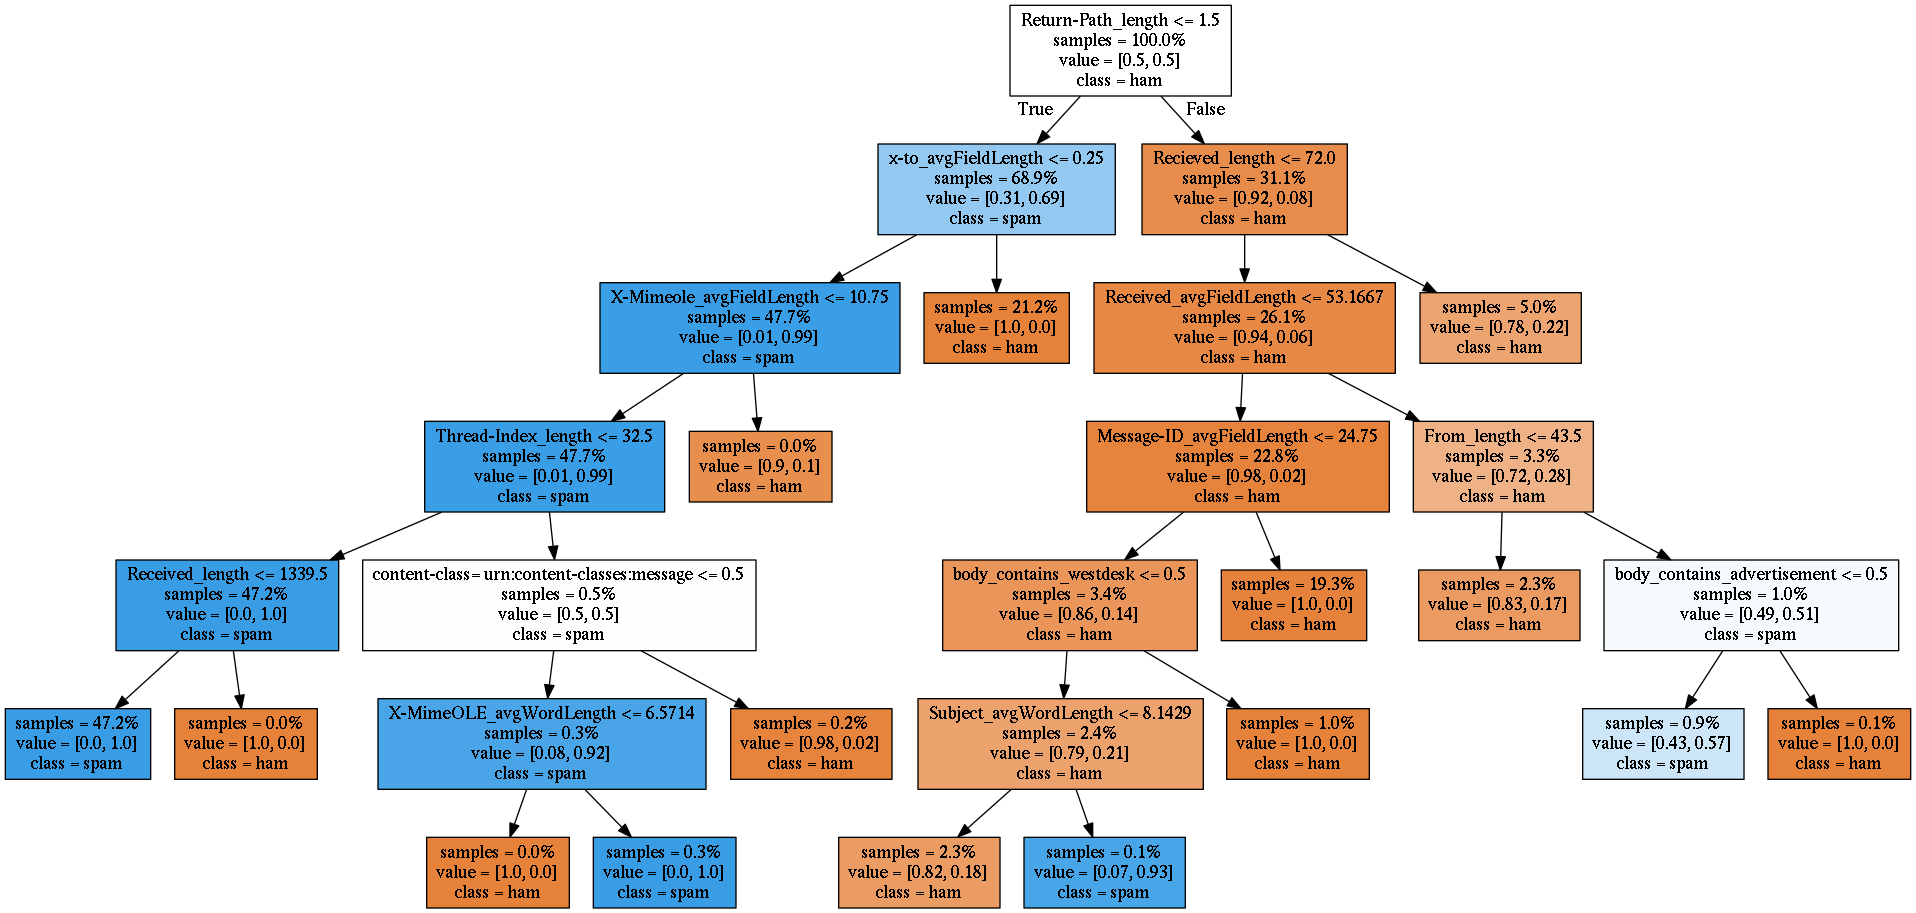
\includegraphics[width=1.3\textwidth]{tree.png}}
	\caption{Árbol de decisión similar con un score un poco menor (pero que es mucho más lindo a la vista).}
\end{figure}

\subsection{Naive Bayes}

Se prueba usar el modelo de Bernoulli usado en sklearn en las variables booleanas del modelo (eso es, todas menos las que hablan de tamaños o de cantidades). Elegimos el parámetro \( \alpha = 1 \) por el simple hecho de que cualquier otro valor daba un peor resultado.

Elegir este modelo aplicando el método de cross validation llega a un score promedio de \( \mathbf{0.952} \).

\section{Reducción de Dimensionalidad}

\section{Resultados}

\section{Discusión}

\end{document}
